\documentclass[aspectratio=169]{beamer}              % only frames

% for themes, etc.
\mode<presentation>
\usetheme{Madrid} 
\usecolortheme{crane}

%\usepackage{times}  % fonts are up to you
% The usual suspects
\usepackage{multirow, booktabs, dcolumn, color, graphicx} % Tables\usepackage{graphicx}
\usepackage{amsmath,amssymb,amsthm}
% Strikethrough text
\usepackage{soul}
% Adjust box to fit tabulars
\usepackage{adjustbox}
% Embed video
\usepackage{media9}
% For notes
\usepackage{pgfpages}
\setbeameroption{hide notes} % Only slides
%\setbeameroption{show only notes} % Only notes
%\setbeameroption{show notes on second screen=right} % Both
% Use colors by name
\usepackage{xcolor}
% EMBEDDING VIDEO IS POSSIBLE WITH PDFPC USE PDF PC to present
\usepackage{multimedia}



% The table highlighting for hypothesis discussion.
\usepackage[beamer,customcolors]{hf-tikz}
\usetikzlibrary{calc}

% To use background images
\newenvironment{colorframe}[2][]{%
\setbeamercolor{background canvas}{bg=#1}
\begin{frame}\color{white}}
{\end{frame}}


% To set the hypothesis highlighting boxes red.
\tikzset{hl/.style={
    set fill color=red!80!black!40,
    set border color=red!80!black,
  },
}

% Set Graphics folder
\graphicspath{{./figures/}}


% these will be used later in the title page
\title{Threatlandscape}
\subtitle{Access: Human Element}
\author{Irfan Kanat}
\institute[CBS]{{Department of Digitization}\\ Copenhagen Business School}
%\date{\today}



\begin{document}

% this prints title, author etc. info from above
\begin{frame}

    \titlepage


    \vfill
    {\tiny \centering This work is licensed under a \href{http://creativecommons.org/licenses/by/4.0/}{Creative Commons Attribution 4.0 International License}.}

\end{frame}

\note{In this presentation we focus on how malicious actors gain access to information assets.}

\begin{frame}
    \frametitle{Big Question}
    
    \large How do they gain access?

\end{frame}

\note{According to DBIR 2021 report, 85\% of the breaches involved some sort of human involvement. In this video we talk about social engineering, a way to exploit the human nature to gain access.}


\begin{frame}
    \frametitle{Human Element}
    
    \centering

    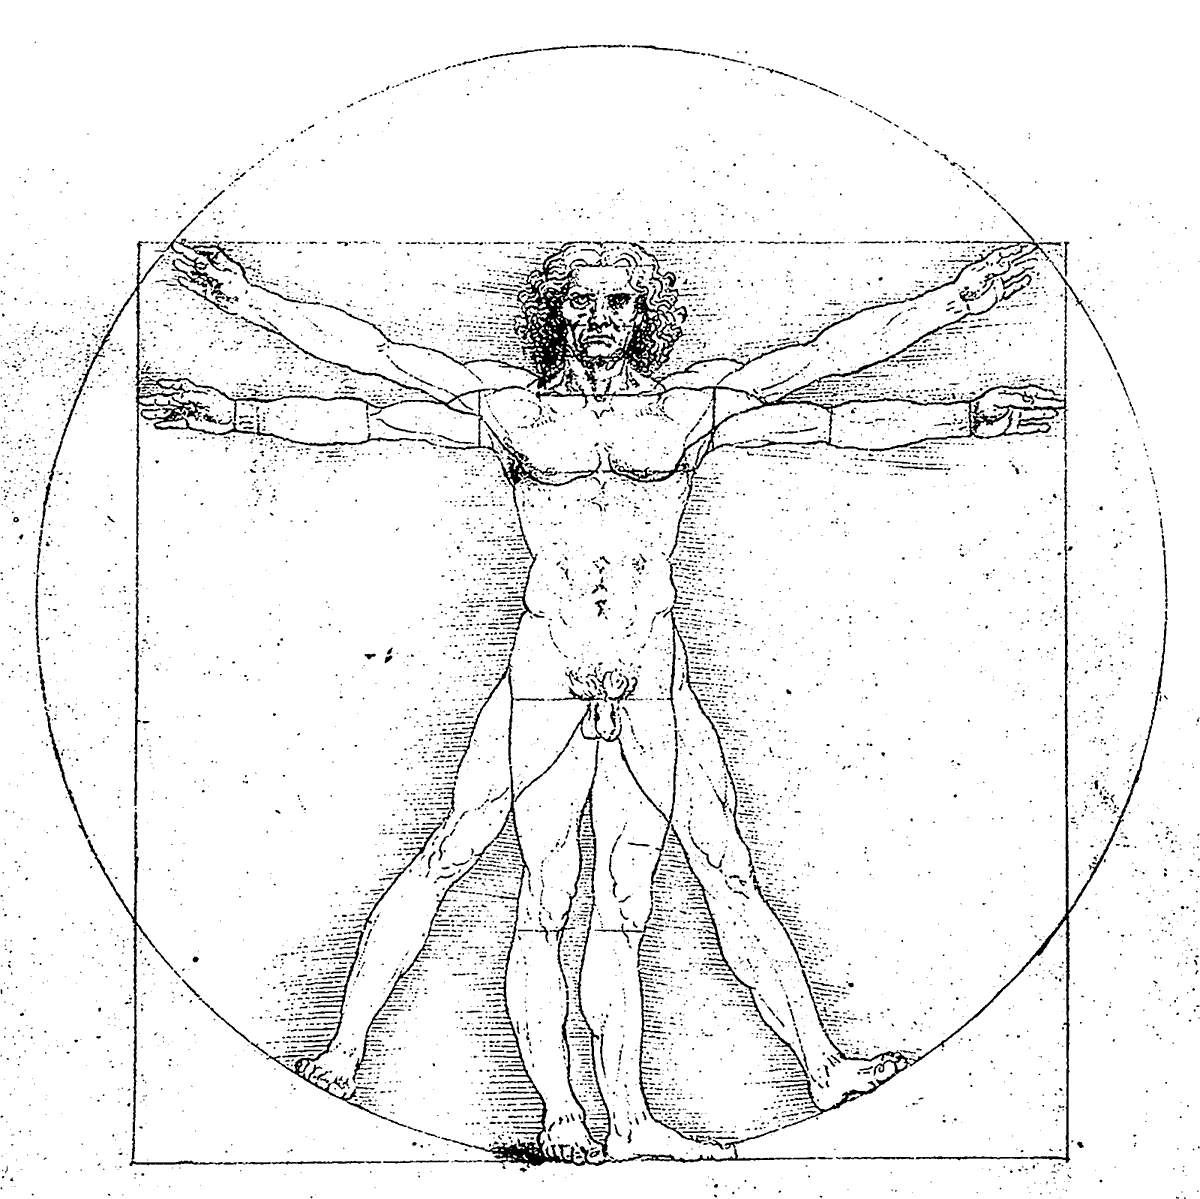
\includegraphics[width = \textwidth, height = .85\textheight, keepaspectratio]{figures/davinci-vitruvian-man.png}

\end{frame}

\note{Installing anti-malware solutions, closing all the ports, using hard to guess passwords are all technical solutions that are increasing the security of your systems. Unfortunately, no matter how tight you lock systems down, it is all for naught if someone from the inside goes about opening those systems up.

We are not necessarily talking about insiders here. People want to be helpful by their nature. Keeping a door open may seem like the polite thing to do but it is a known tactic to piggy back on other people to gain access to restricted areas.}

\begin{frame}
    \frametitle{Social Engineering}

    \centering
    
    \movie{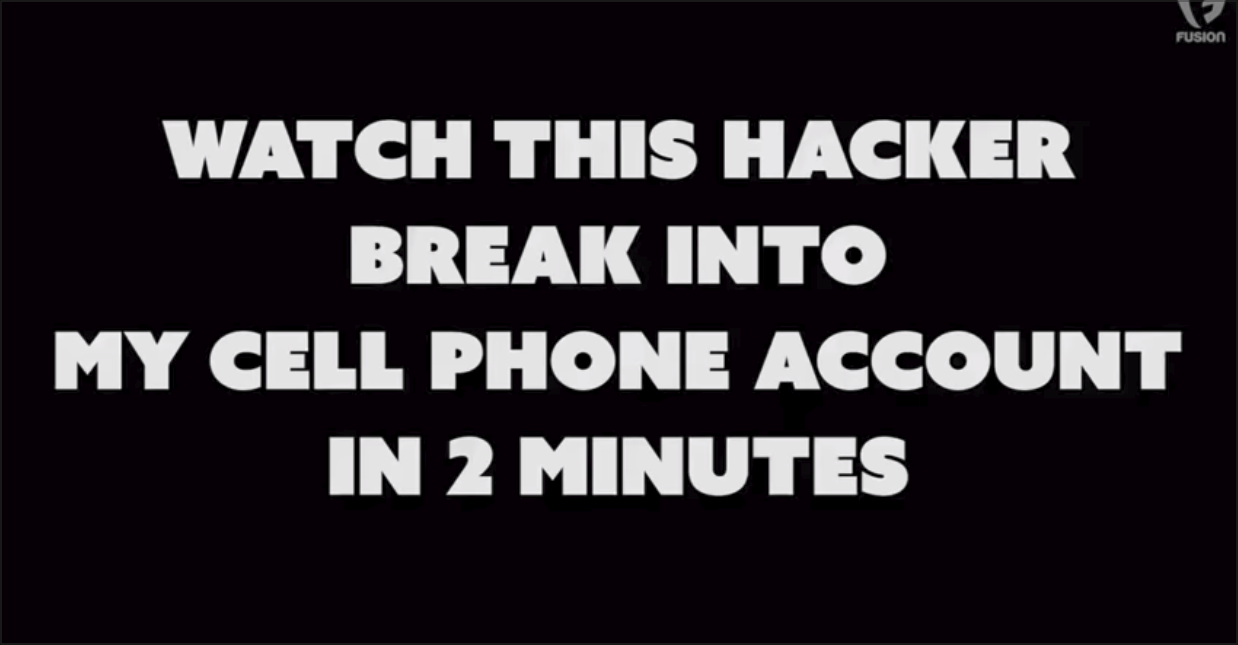
\includegraphics[width = \textwidth]{figures/SocEng.png}}{figures/SocEng.mp4}

\end{frame}

\note{Social engineering is the practice of exploiting human nature to gain access to information. Its proponents call it a forever day vulnerability.}

\begin{frame}
    \frametitle{What to Do?}
    
    \centering

    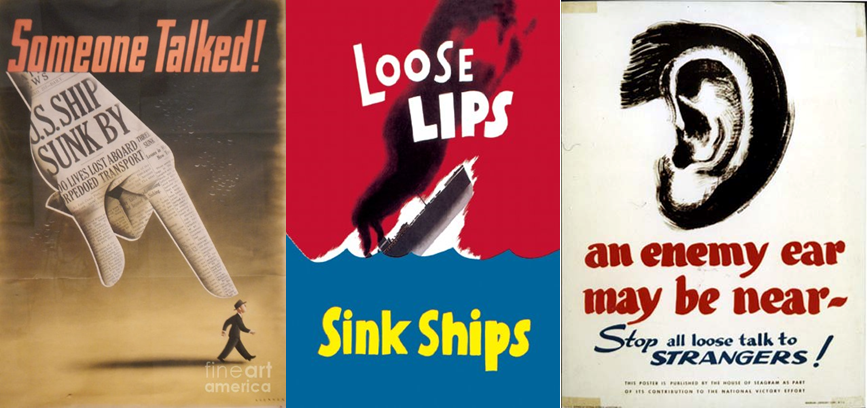
\includegraphics[width = \textwidth, height = .85\textheight, keepaspectratio]{figures/carelessWhisper.png}

\end{frame}

\note{As individuals we should be careful about what information we divulge. As organizations, we should make sure our employees are constantly reminded of security implications of their behavior. This is covered in awareness training.

Furthermore, the employees that have access to critical information and systems should receive training appropriate for their role.}


\end{document}
